\documentclass[preprint,12pt,authoryear]{elsarticle}

\usepackage{amsmath,amssymb,amsfonts}
\usepackage{graphicx}
\usepackage{booktabs}
\usepackage{multirow}
\usepackage{url}
\usepackage{microtype}
\usepackage{hyperref}
\usepackage{geometry}
\geometry{a4paper, margin=1in}

\journal{Computational Biology and Chemistry}

\begin{document}

\begin{frontmatter}

\title{Sequence-Only Protein Secondary Structure Prediction under a CPU Budget: Accuracy--Latency Trade-offs of Frozen ESM-2 Probes and Lightweight Non-Pretrained Networks}

\author[inst1]{Roaissat Mohamed Zakaria\corref{cor1}}
\ead{roaissatmohamedzakaria@gmail.com}

\cortext[cor1]{Corresponding author.}
\affiliation[inst1]{organization={Independent Researcher},
            country={Algeria}}

\begin{abstract}
Accurate protein secondary structure prediction (PSSP) traditionally relies on evolutionary profiles from multiple sequence alignments (MSAs), whose database searches dominate run time. We present a reproducible, multi-seed benchmark of five MSA-free predictors that differ by orders of magnitude in cost: a windowed multilayer perceptron (WindowMLP), a hybrid 1D-CNN--BiLSTM, and frozen ESM-2 protein language models (8M and 35M parameters) with linear or MLP classification heads. All models were trained on the NetSurfP-2.0 training set after removing every chain with $\geq 25\%$ identity to any test chain (MMseqs2), and evaluated on CB513, TS115, CASP12, CASP13 and CASP14 over three seeds. On CB513, $Q_3$ rose from $67.95 \pm 0.05\%$ (WindowMLP) and $71.45 \pm 0.22\%$ (hybrid) to $75.92 \pm 0.03\%$ (frozen ESM-2 8M + MLP head) and $80.12 \pm 0.05\%$ (frozen ESM-2 35M + MLP head). Replacing a linear probe with a 20,739-parameter MLP head added $+1.61$ points. On a two-thread CPU, the hybrid network ran $5.8\times$ faster than the ESM-2 8M pipeline (14.2 vs.\ 82.6\,ms per sequence) with $10.8\times$ fewer parameters, but recovered only $43.9\%$ of the accuracy gain of ESM-2 8M over WindowMLP; ESM-2 35M added $+4.20$ points at $4.0\times$ the CPU latency of ESM-2 8M. All pairwise differences were significant in residue-level McNemar, protein-level Wilcoxon and protein-level bootstrap tests. Pretrained models lost more accuracy than non-pretrained ones from CB513 to the small CASP12 and CASP14 sets, a pattern that warrants caution when interpreting CB513 results for language-model-based predictors.
\end{abstract}

\begin{graphicalabstract}
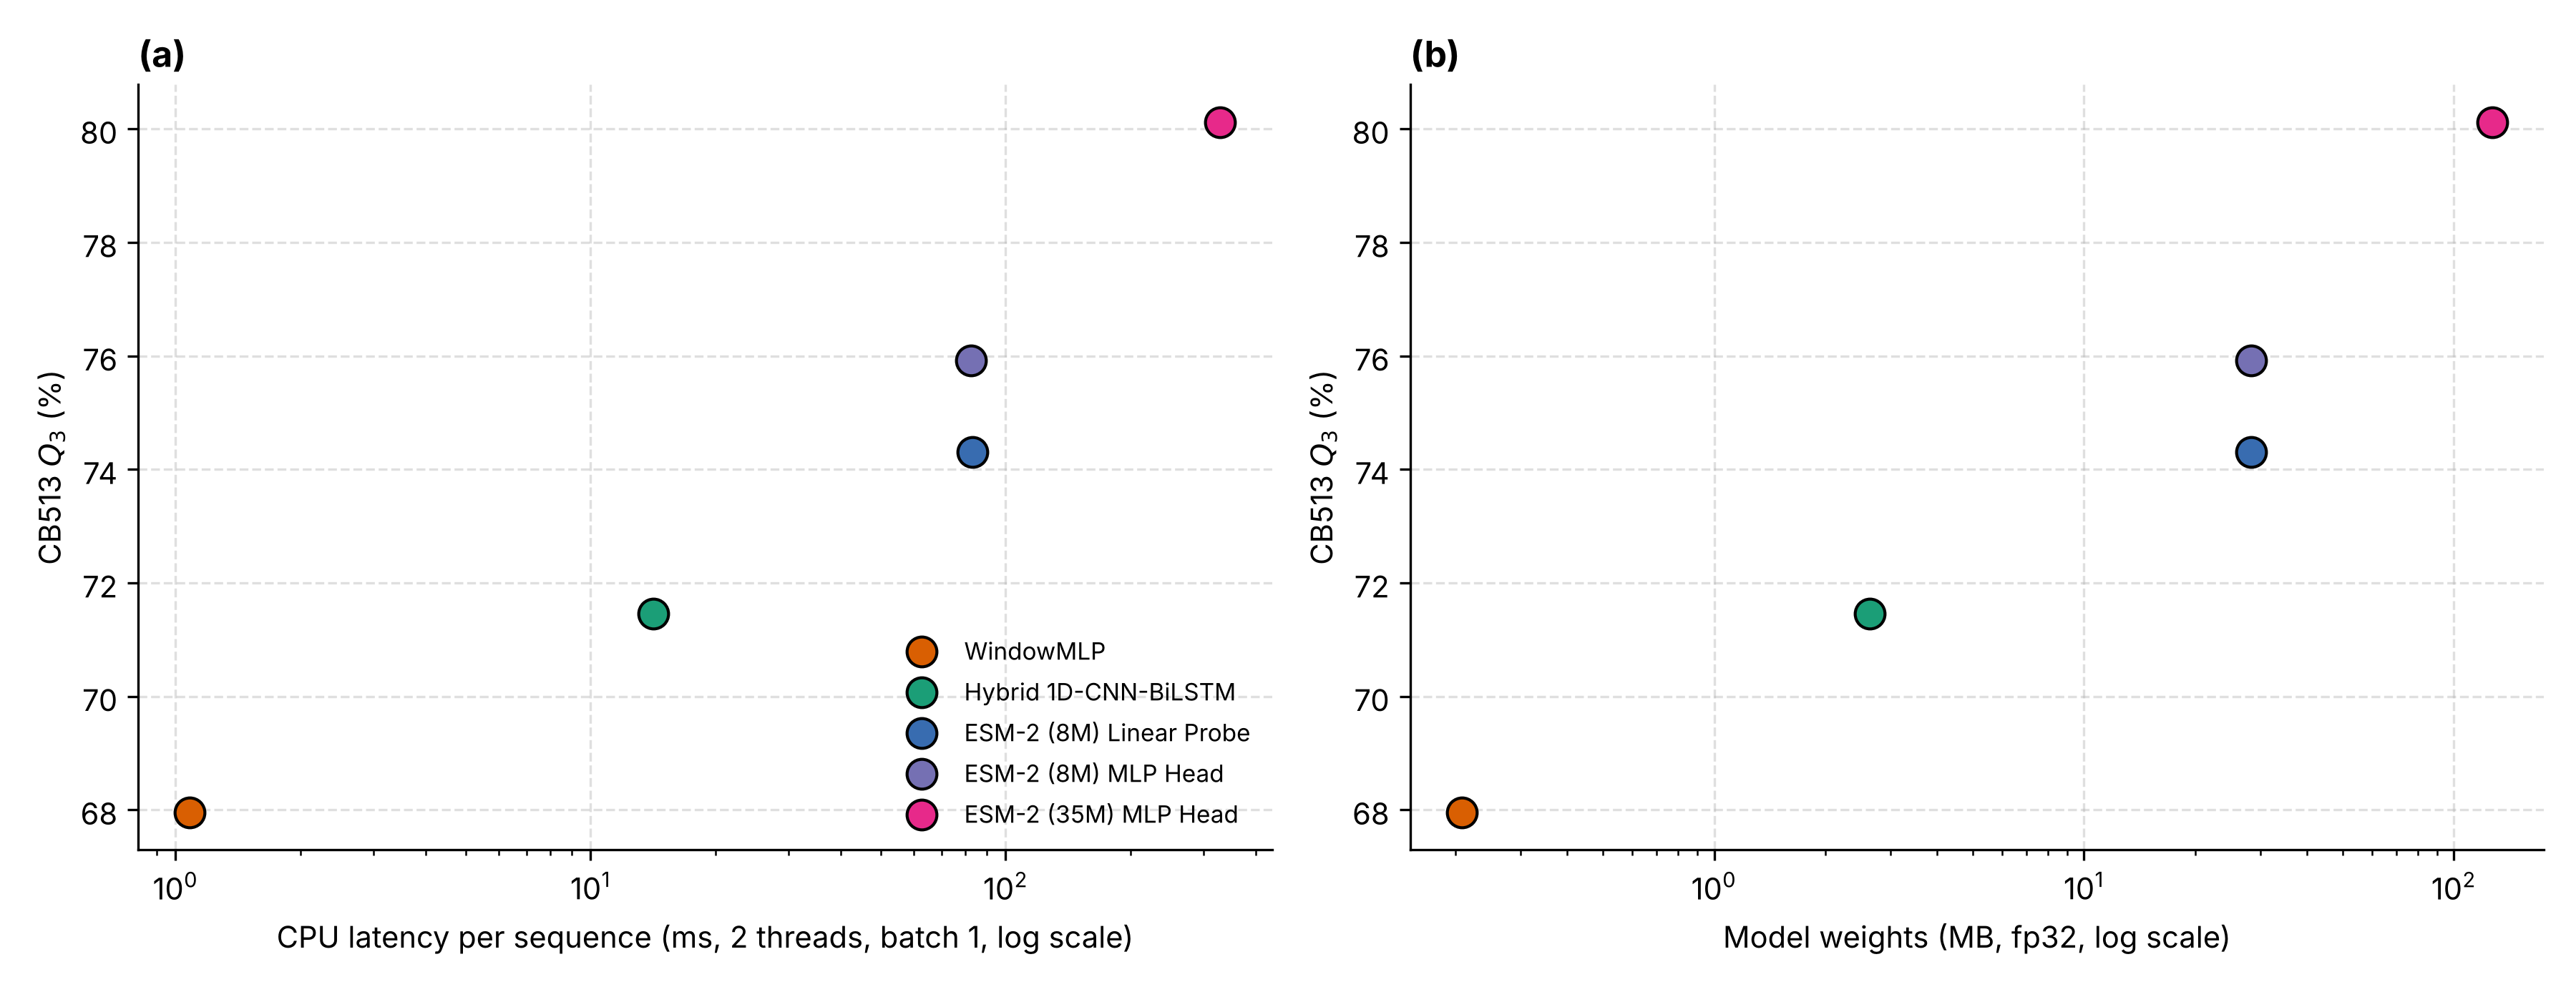
\includegraphics[width=\textwidth]{results_real/fig_pareto.png}
\end{graphicalabstract}

\begin{highlights}
\item Five MSA-free secondary structure predictors benchmarked on five test sets.
\item Training chains with $\geq$25\% identity to any test chain removed by MMseqs2.
\item Frozen ESM-2 35M with an MLP head reaches 80.12\% Q3 on CB513.
\item Hybrid CNN-BiLSTM is 5.8x faster than ESM-2 8M on CPU but 4.5 points lower.
\item Pretrained models drop more than baselines from CB513 to CASP12/CASP14.
\end{highlights}

\begin{keyword}
Protein secondary structure prediction \sep MSA-free \sep ESM-2 \sep Frozen-backbone probing \sep CPU inference \sep Benchmark
\end{keyword}

\end{frontmatter}

%======================================================================
\section{Introduction}
\label{sec:intro}
Assigning each residue of a protein to helix ($H$), strand ($E$) or coil ($C$) is a long-standing intermediate task in structural bioinformatics~\citep{rost1993prediction,kabsch1983dictionary}. For three decades the most accurate predictors have used evolutionary profiles derived from multiple sequence alignments (MSAs), as in PSIPRED~\citep{jones1999protein,buchan2019psipred}, JPred4~\citep{drozdetskiy2015jpred4} and NetSurfP-2.0~\citep{klausen2019netsurfp}. Profile construction requires iterative database searches that dominate the run time and degrade for sequences with few homologues, such as orphan or designed proteins~\citep{singh2021spot1d,elnaggar2022prottrans}.

Single-sequence (MSA-free) predictors avoid this step. They range from networks trained only on one-hot or physicochemical encodings~\citep{singh2021spot1d} to predictors built on protein language models (pLMs) such as ESM-1b, ESM-2 and ProtT5~\citep{rives2021biological,lin2023evolutionary,elnaggar2022prottrans,hoie2022netsurfp3}. Large pLMs approach MSA-based accuracy but are expensive to run, which matters for users without GPUs and for screening large sequence collections.

This work does not propose a new architecture. It is a controlled benchmark of the accuracy--cost trade-off of small MSA-free predictors that can run on a commodity CPU. We ask four questions:
\begin{enumerate}
    \item How much accuracy do frozen embeddings from the two smallest ESM-2 models (8M and 35M parameters) provide over non-pretrained networks trained on the same data?
    \item How much does a small non-linear (MLP) head add over a linear probe on the same frozen embeddings?
    \item Where does a compact hybrid CNN--BiLSTM sit on the accuracy--latency frontier?
    \item Are the conclusions stable across benchmarks of different age and size (CB513, TS115, CASP12--14)?
\end{enumerate}

%======================================================================
\section{Materials and Methods}
\label{sec:methods}

\subsection{Data and homology filtering}
We used the NetSurfP-2.0 training set and the CB513~\citep{cuff1999evaluation}, TS115~\citep{yang2018sixty}, CASP12, CASP13 and CASP14 test sets as distributed in the public Hugging Face dataset \texttt{proteinea/secondary\_structure\_prediction} (DOI 10.57967/hf/1104), which provides sequences, 8-state DSSP labels and per-residue evaluation masks. The training file contained 10,792 chains.

To remove homology between training and test data, we searched all test chains against all training chains with MMseqs2 (\texttt{easy-search}, sensitivity 7.5, E-value $\leq 10^{-3}$) and removed every training chain that aligned to any test chain with $\geq 25\%$ sequence identity and $\geq 50\%$ coverage of both sequences. Hits were found for 205 CB513 and 49 TS115 query chains and for none of the CASP chains; 202 training chains were removed, leaving 10,590. These were split once at random (seed 0) into 9,531 training chains (2,437,114 residues) and 1,059 validation chains; the same split was used for all models and seeds. The validation set was used only for early stopping.

Eight-state DSSP labels were reduced to three states as $H \leftarrow \{H,G,I\}$, $E \leftarrow \{E,B\}$ and $C \leftarrow$ all other states. Following the dataset's masks, only residues flagged as structurally resolved were scored (for CB513, additionally only residues inside the CB513 mask). Table~\ref{tab:data} lists the evaluated sets. The three CASP sets are small (12--20 chains), so their results carry substantial sampling uncertainty that is not captured by the seed standard deviations.

\begin{table}[htbp]
\centering
\small
\caption{Evaluation sets after masking. Chains: chains with at least one evaluated residue.}
\label{tab:data}
\begin{tabular}{lrr}
\toprule
\textbf{Set} & \textbf{Chains} & \textbf{Evaluated residues} \\
\midrule
CB513  & 509 & 83,427 \\
TS115  & 115 & 27,501 \\
CASP12 & 20  & 6,004 \\
CASP13 & 12  & 2,280 \\
CASP14 & 18  & 2,718 \\
\bottomrule
\end{tabular}
\end{table}

\subsection{Models}
All models were implemented in PyTorch and trained with three seeds (42, 123, 2026), which control weight initialisation and data order. Exact hyper-parameters are listed in Table~\ref{tab:hyperparams}. All models were trained with per-residue cross-entropy, early stopping on validation loss, and the checkpoint with the lowest validation loss was evaluated.

\paragraph{WindowMLP} Each residue is represented by a symmetric window of 17 residues, one-hot encoded with 21 channels (20 amino acids plus one channel for unknown residues and padding), giving 357 inputs. The network is Linear(357$\to$128)--BatchNorm--ReLU--Dropout(0.2)--Linear(128$\to$64)--BatchNorm--ReLU--Dropout(0.2)--Linear(64$\to$3); the two linear layers that precede batch normalisation have no bias. It has 54,467 trainable parameters.

\paragraph{Hybrid 1D-CNN--BiLSTM} The one-hot sequence (21 channels) passes through three parallel 1D convolutions with kernel sizes 3, 5 and 7 (42, 42 and 44 channels; 128 in total), BatchNorm, ReLU and channel-wise (spatial) dropout ($p=0.3$), then a two-layer bidirectional LSTM (hidden size 128 per direction, inter-layer dropout 0.3) on packed sequences, LayerNorm(256), and a head Linear(256$\to$64)--ReLU--Dropout(0.3)--Linear(64$\to$3). It has 690,519 trainable parameters.

\paragraph{Frozen ESM-2 probes} We used \texttt{facebook/esm2\_t6\_8M\_UR50D} (6 layers, 20 attention heads, hidden size 320) and \texttt{facebook/esm2\_t12\_35M\_UR50D} (12 layers, 20 heads, hidden size 480)~\citep{lin2023evolutionary}. The backbones were loaded without the language-model head and pooling layer (7,409,081 and 33,269,521 parameters) and kept frozen. Per-residue embeddings from the last layer were computed once (mixed precision, float16 storage); chains longer than 1,022 residues were embedded in consecutive 1,022-residue segments. Two heads were trained on these embeddings: a linear probe, Linear($d \to 3$) (963 parameters for $d=320$), and an MLP head, Linear($d \to 64$)--ReLU--Dropout(0.2)--Linear(64$\to$3) (20,739 parameters for $d=320$; 30,979 for $d=480$). Because the head is applied independently to each residue, heads were trained on shuffled mini-batches of 4,096 residues.

\begin{table*}[htbp]
\centering
\small
\caption{Training hyper-parameters. Batch sizes are in sequences for WindowMLP and the hybrid model, and in residues for the ESM-2 heads. Epochs: epochs run / epoch of the selected checkpoint, for seeds 42, 123 and 2026.}
\label{tab:hyperparams}
\resizebox{\textwidth}{!}{%
\begin{tabular}{lccccccc}
\toprule
\textbf{Model} & \textbf{Optimizer} & \textbf{LR} & \textbf{Weight decay} & \textbf{Batch} & \textbf{Max epochs} & \textbf{Patience} & \textbf{Epochs (run / best)} \\
\midrule
WindowMLP & Adam & $10^{-3}$ & $10^{-4}$ & 32 seq. & 20 & 3 & 16/13, 17/14, 17/14 \\
Hybrid 1D-CNN--BiLSTM & AdamW & $10^{-3}$ & $10^{-4}$ & 16 seq. & 20 & 3 & 15/12, 19/16, 10/7 \\
ESM-2 (8M) linear probe & Adam & $10^{-3}$ & 0 & 4,096 res. & 30 & 4 & 11/7, 14/14, 12/12 \\
ESM-2 (8M) MLP head & Adam & $10^{-3}$ & 0 & 4,096 res. & 30 & 4 & 28/25, 23/23, 18/15 \\
ESM-2 (35M) MLP head & Adam & $10^{-3}$ & 0 & 4,096 res. & 30 & 4 & 21/17, 24/21, 28/24 \\
\bottomrule
\end{tabular}}
\end{table*}

\subsection{Evaluation metrics}
\begin{enumerate}
    \item \textbf{$Q_3$}: percentage of correctly predicted evaluated residues, pooled over all chains of a test set.
    \item \textbf{SOV'99}: the segment overlap score of \citet{zemla1999modified}, computed per chain on the evaluated residues and averaged over chains.
    \item \textbf{Macro-F1}: unweighted mean of the per-class F1 scores.
    \item \textbf{$\beta$--coil error}: (true $E$ predicted as $C$ + true $C$ predicted as $E$) / (true $E$ + true $C$), in percent.
    \item \textbf{Cost}: total and trainable parameters; size of the fp32 weights; and end-to-end latency per sequence at batch size 1, measured from the amino-acid string (including encoding or tokenisation) on the first 100 (GPU) or 50 (CPU) CB513 chains after three warm-up calls. CPU timings used two threads and were measured once (seed 42); GPU timings are averaged over seeds. For timing, ESM-2 inputs were truncated to 1,022 residues.
\end{enumerate}
All experiments ran on Google Colab with an NVIDIA Tesla T4 GPU and an Intel Xeon CPU at 2.00\,GHz (2 vCPUs), using Python 3.13.16, PyTorch 2.14.1 (CUDA 13.0) and Transformers 5.22.1.

\subsection{Statistical tests}
Paired comparisons used the CB513 predictions of seed 42 (83,427 residues, 509 chains). We report (i) McNemar's test with continuity correction on residue-level correct/incorrect outcomes; (ii) a two-sided Wilcoxon signed-rank test on per-chain $Q_3$; and (iii) a paired bootstrap over whole chains ($B=10{,}000$) of the difference in pooled $Q_3$, which accounts for the correlation of residues within a chain. The bootstrap $p$-value is two-sided; when no resample crossed zero we report $p \leq 1/B$.

%======================================================================
\section{Results}
\label{sec:results}

\subsection{Accuracy across benchmarks}
Table~\ref{tab:results} and Fig.~\ref{fig:benchmarks} summarise accuracy. The ranking WindowMLP $<$ hybrid $<$ ESM-2 (8M) linear $<$ ESM-2 (8M) MLP $<$ ESM-2 (35M) MLP held on CB513, TS115, CASP12 and CASP13. On CASP14 the ESM-2 (8M) linear probe and MLP head were practically tied ($72.66\%$ vs.\ $72.79\%$). Seed-to-seed variation was small for the frozen-backbone probes ($\leq 0.20$ points in $Q_3$ on every set) because only the head is trained; it was larger for the hybrid network on the small CASP13 and CASP14 sets ($1.79$ and $0.96$ points).

\begin{table*}[htbp]
\centering
\scriptsize
\caption{Accuracy (mean $\pm$ SD over three seeds). SOV'99, macro-F1 and $\beta$--coil error are on CB513.}
\label{tab:results}
\resizebox{\textwidth}{!}{%
\begin{tabular}{lcccccccc}
\toprule
\textbf{Model} & \textbf{CB513 $Q_3$} & \textbf{CB513 SOV'99} & \textbf{TS115 $Q_3$} & \textbf{CASP12 $Q_3$} & \textbf{CASP13 $Q_3$} & \textbf{CASP14 $Q_3$} & \textbf{Macro-F1} & \textbf{$\beta$--coil err.} \\
\midrule
WindowMLP & $67.95 \pm 0.05$ & $62.02 \pm 0.25$ & $70.20 \pm 0.11$ & $66.87 \pm 0.50$ & $66.62 \pm 0.40$ & $66.54 \pm 0.22$ & $66.44 \pm 0.06$ & $18.86 \pm 0.02$ \\
Hybrid 1D-CNN--BiLSTM & $71.45 \pm 0.22$ & $67.66 \pm 0.40$ & $73.87 \pm 0.36$ & $69.83 \pm 0.30$ & $72.03 \pm 1.79$ & $71.56 \pm 0.96$ & $70.42 \pm 0.21$ & $18.45 \pm 0.20$ \\
ESM-2 (8M) linear probe & $74.31 \pm 0.02$ & $67.46 \pm 0.10$ & $77.13 \pm 0.01$ & $72.30 \pm 0.11$ & $76.80 \pm 0.08$ & $72.66 \pm 0.20$ & $73.53 \pm 0.02$ & $17.43 \pm 0.02$ \\
ESM-2 (8M) MLP head & $75.92 \pm 0.03$ & $70.08 \pm 0.34$ & $78.73 \pm 0.04$ & $73.30 \pm 0.23$ & $78.19 \pm 0.17$ & $72.79 \pm 0.20$ & $75.17 \pm 0.06$ & $16.34 \pm 0.02$ \\
ESM-2 (35M) MLP head & $\mathbf{80.12 \pm 0.05}$ & $\mathbf{74.45 \pm 0.13}$ & $\mathbf{81.88 \pm 0.08}$ & $\mathbf{74.84 \pm 0.05}$ & $\mathbf{80.44 \pm 0.04}$ & $\mathbf{74.76 \pm 0.17}$ & $\mathbf{79.60 \pm 0.04}$ & $\mathbf{14.17 \pm 0.09}$ \\
\bottomrule
\end{tabular}}
\end{table*}

\begin{figure}[htbp]
\centering
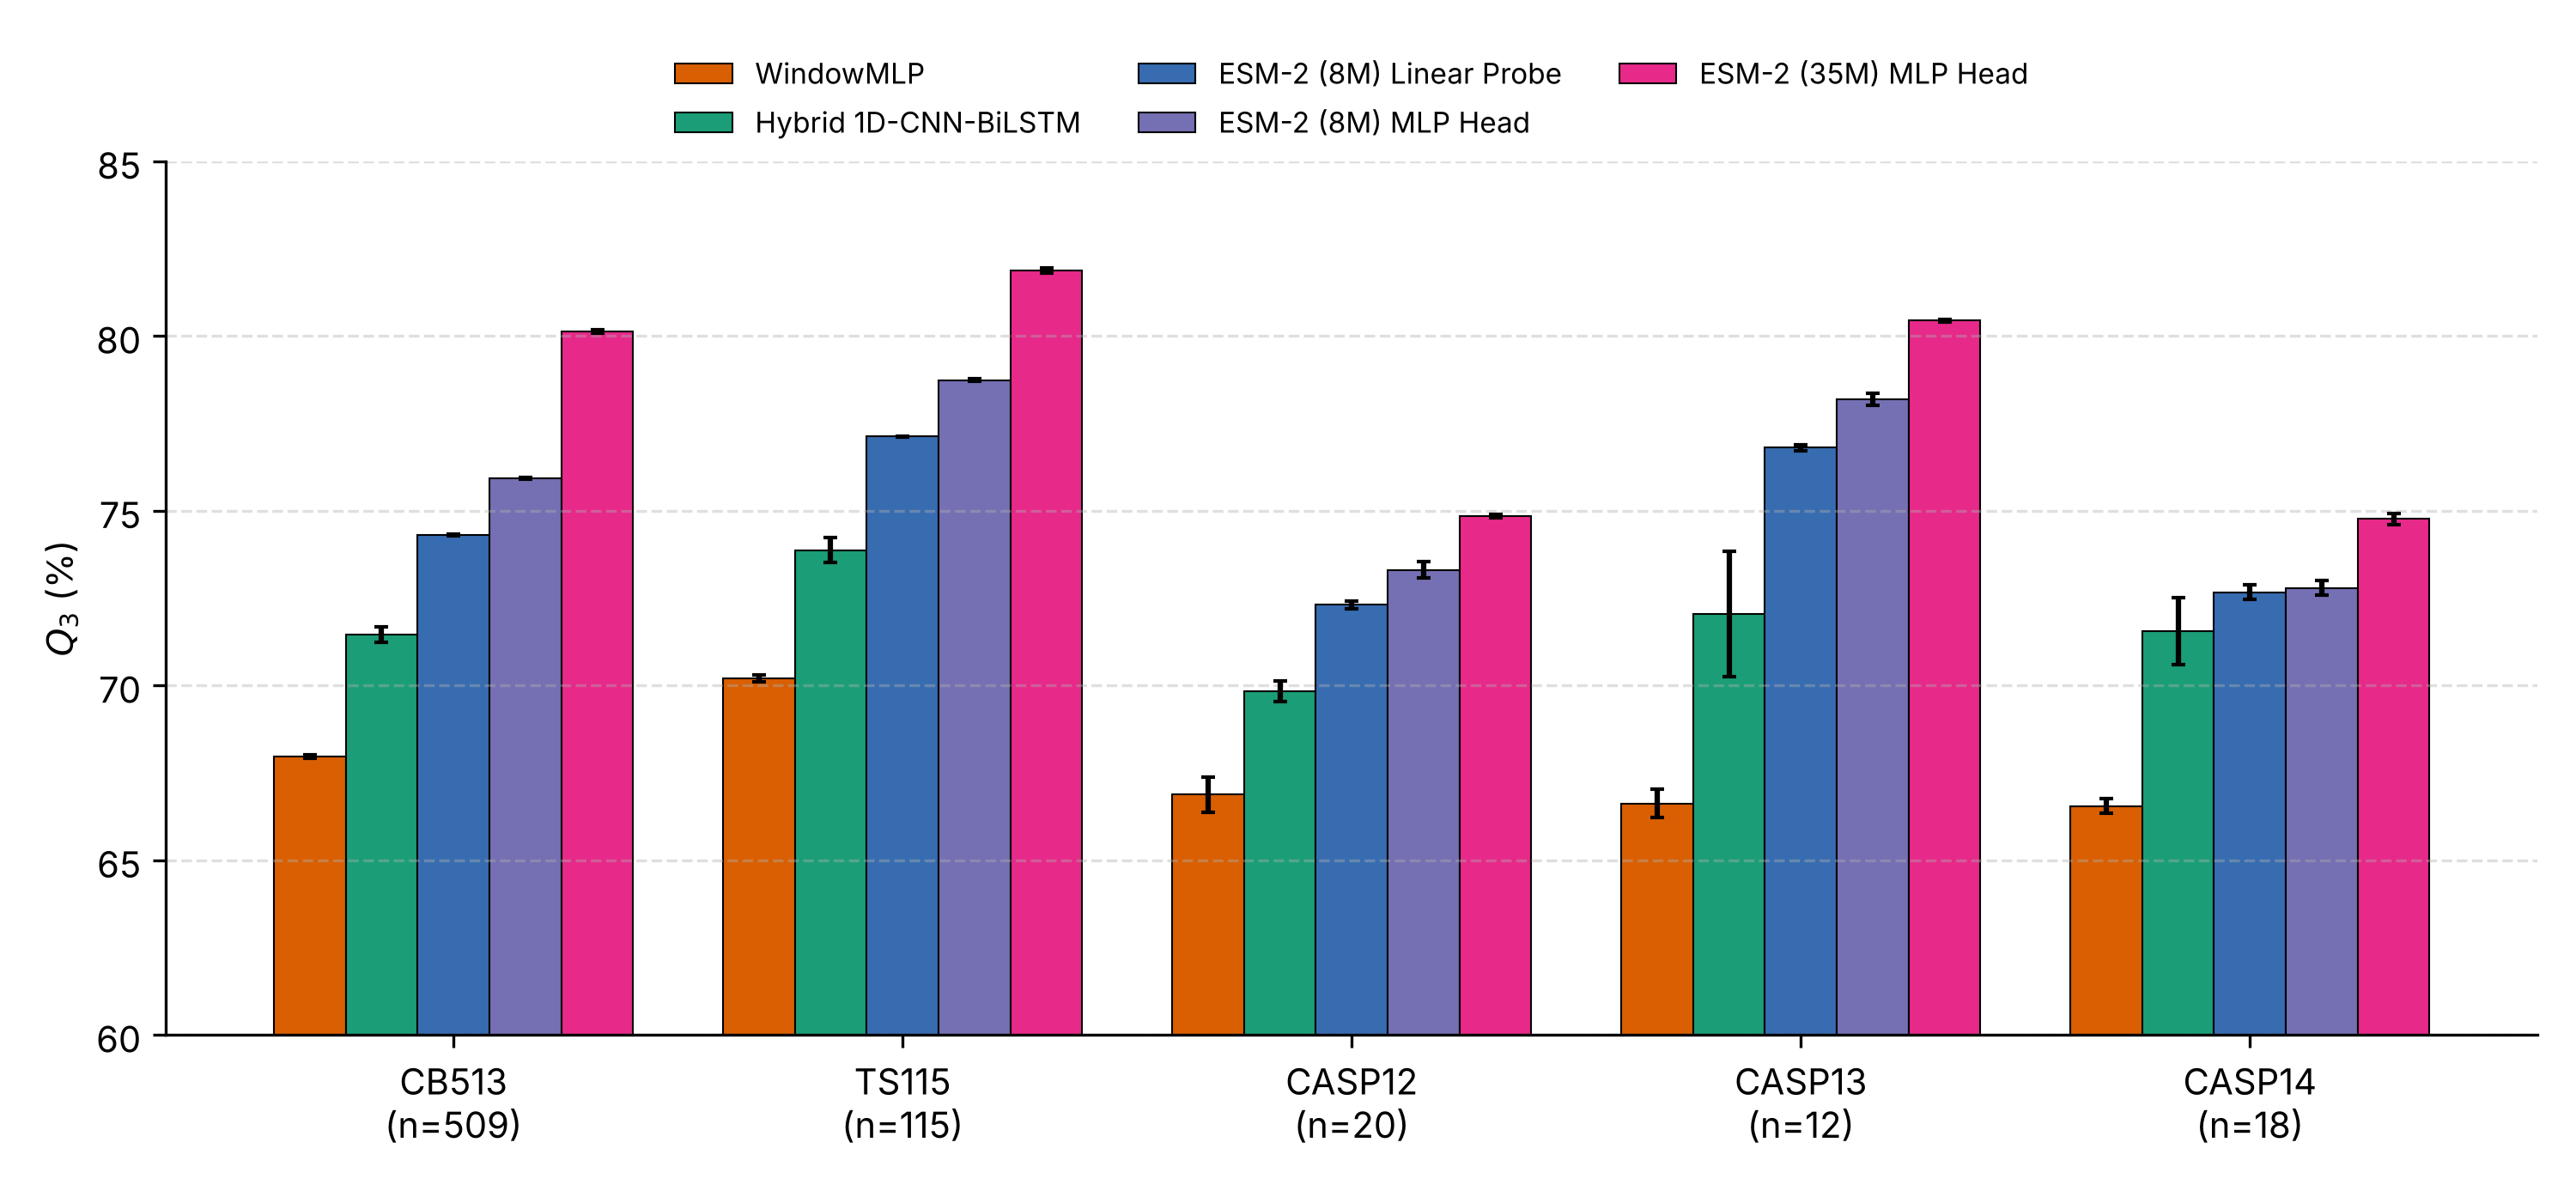
\includegraphics[width=0.98\linewidth]{results_real/fig_benchmarks.png}
\caption{$Q_3$ on the five test sets (mean $\pm$ SD over three seeds; $n$ = evaluated chains).}
\label{fig:benchmarks}
\end{figure}

\subsection{Effect of the head and of backbone size}
On frozen ESM-2 (8M) embeddings, the MLP head improved CB513 $Q_3$ over the linear probe by $+1.61$ points ($74.31\% \to 75.92\%$), SOV'99 by $+2.62$ points, and reduced the $\beta$--coil error from $17.43\%$ to $16.34\%$. The gain was consistent on TS115 ($+1.60$), CASP12 ($+1.00$) and CASP13 ($+1.39$), but negligible on CASP14 ($+0.13$). Moving from the 8M to the 35M backbone with the same head type added $+4.20$ points on CB513 and reduced the $\beta$--coil error to $14.17\%$. For every model, most $\beta$--coil errors were strands predicted as coil (Table~\ref{tab:perclass}).

\begin{table}[htbp]
\centering
\scriptsize
\caption{Per-class F1 and directional $E/C$ confusion on CB513 (mean over three seeds, \%).}
\label{tab:perclass}
\begin{tabular}{lccccc}
\toprule
\textbf{Model} & \textbf{F1$_H$} & \textbf{F1$_E$} & \textbf{F1$_C$} & \textbf{$E\to C$} & \textbf{$C\to E$} \\
\midrule
WindowMLP & 71.63 & 57.42 & 70.28 & 29.69 & 13.18 \\
Hybrid 1D-CNN--BiLSTM & 76.05 & 63.32 & 71.90 & 28.65 & 13.10 \\
ESM-2 (8M) linear probe & 79.07 & 67.71 & 73.80 & 29.49 & 11.11 \\
ESM-2 (8M) MLP head & 80.37 & 69.60 & 75.54 & 28.08 & 10.18 \\
ESM-2 (35M) MLP head & 84.41 & 75.22 & 79.18 & 25.44 & 8.26 \\
\bottomrule
\end{tabular}
\end{table}

\subsection{Cost and the accuracy--latency frontier}
Table~\ref{tab:cost} and Fig.~\ref{fig:pareto} relate accuracy to cost. On CPU, latency spanned more than two orders of magnitude, from 1.08\,ms per sequence (WindowMLP) to 329.08\,ms (ESM-2 35M). The hybrid network ran $5.8\times$ faster than the ESM-2 (8M) pipeline (14.18 vs.\ 82.55\,ms) and had $10.8\times$ fewer parameters (690,519 vs.\ 7,429,820), but was $4.47$ points less accurate on CB513; it recovered $43.9\%$ of the $Q_3$ gain of ESM-2 (8M) + MLP over WindowMLP ($3.50$ of $7.97$ points). ESM-2 (35M) was $4.0\times$ slower than ESM-2 (8M) on CPU and $4.5\times$ larger in weights.

On the T4 GPU the ordering differed: the batch-size-1 BiLSTM (14.52\,ms) was slower than the ESM-2 (8M) pipeline (8.83\,ms), because the recurrent layers process residues sequentially. The speed advantage of the hybrid model is therefore specific to CPU deployment.

\begin{table*}[htbp]
\centering
\scriptsize
\caption{Model size and end-to-end inference latency at batch size 1. GPU: mean $\pm$ SD over three seeds; CPU: single run (seed 42), two threads. Total parameters include the frozen ESM-2 backbone.}
\label{tab:cost}
\resizebox{\textwidth}{!}{%
\begin{tabular}{lrrrcrc}
\toprule
\textbf{Model} & \textbf{Total params} & \textbf{Trainable params} & \textbf{Weights (MB, fp32)} & \textbf{GPU latency (ms)} & \textbf{CPU latency (ms)} & \textbf{CPU throughput (seq/s)} \\
\midrule
WindowMLP & 54,467 & 54,467 & 0.21 & $1.13 \pm 0.21$ & 1.08 & 924.2 \\
Hybrid 1D-CNN--BiLSTM & 690,519 & 690,519 & 2.63 & $14.52 \pm 0.28$ & 14.18 & 70.5 \\
ESM-2 (8M) linear probe & 7,410,044 & 963 & 28.27 & $10.16 \pm 1.59$ & 83.05 & 12.0 \\
ESM-2 (8M) MLP head & 7,429,820 & 20,739 & 28.34 & $8.83 \pm 0.72$ & 82.55 & 12.1 \\
ESM-2 (35M) MLP head & 33,300,500 & 30,979 & 127.03 & $18.29 \pm 2.07$ & 329.08 & 3.0 \\
\bottomrule
\end{tabular}}
\end{table*}

\begin{figure*}[htbp]
\centering
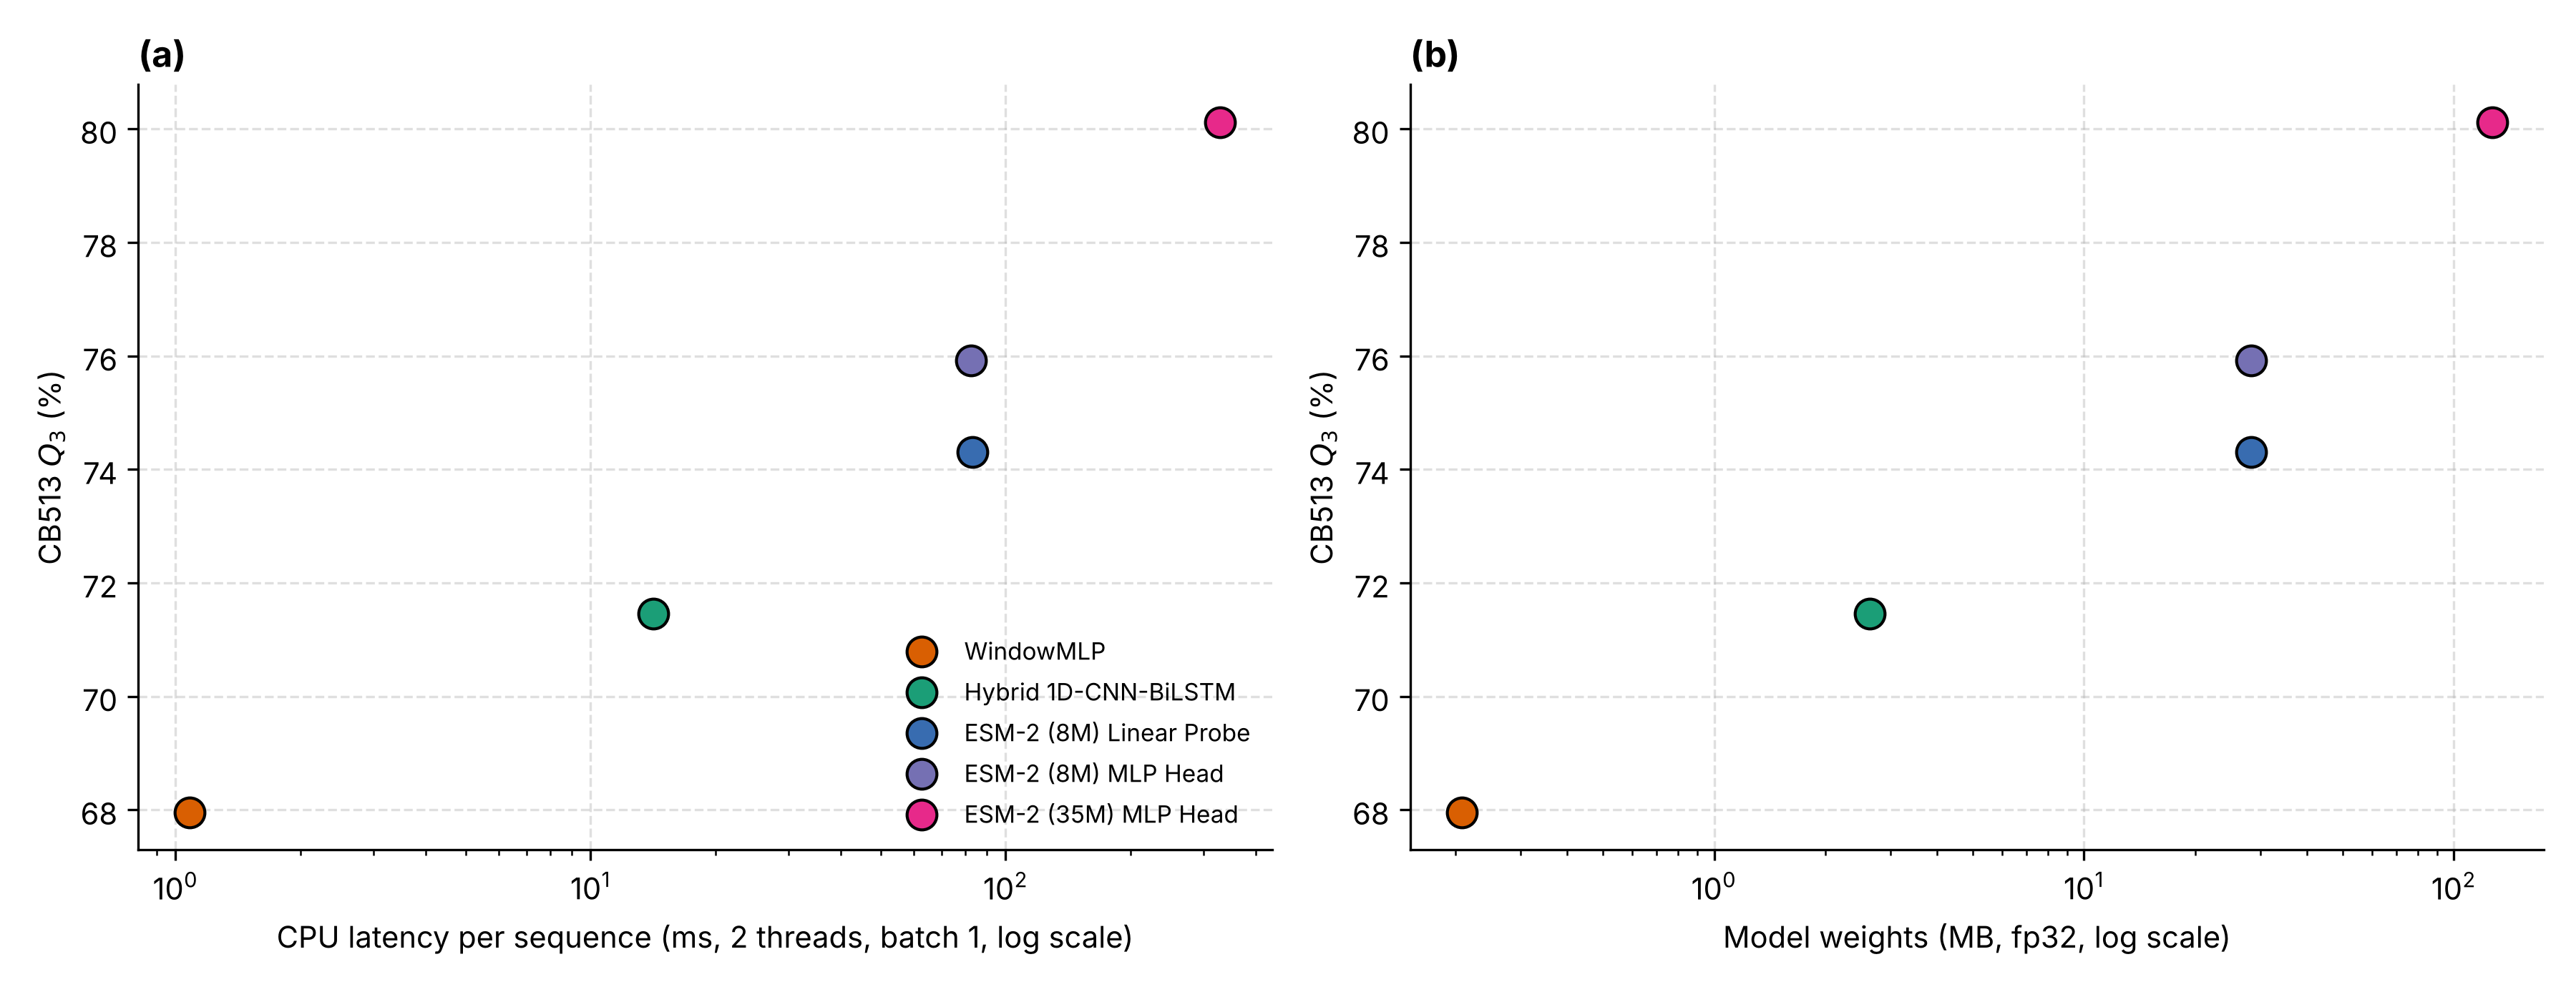
\includegraphics[width=0.98\textwidth]{results_real/fig_pareto.png}
\caption{Accuracy--cost trade-off on CB513: (a) $Q_3$ vs.\ CPU latency per sequence (two threads, batch size 1); (b) $Q_3$ vs.\ fp32 weight size. Error bars: SD of $Q_3$ over three seeds (smaller than the markers).}
\label{fig:pareto}
\end{figure*}

\subsection{Statistical significance}
All three paired comparisons were significant under every test (Table~\ref{tab:stats}). The chain-level bootstrap intervals were wide relative to the seed standard deviations, showing that, on a test set of this size, sampling of chains rather than training randomness dominates the uncertainty of the estimated differences.

\begin{table*}[htbp]
\centering
\scriptsize
\caption{Paired tests on CB513 (seed 42; 83,427 residues; 509 chains). $\Delta Q_3$: difference in pooled $Q_3$ (A $-$ B) with its 95\% chain-level bootstrap interval ($B=10{,}000$).}
\label{tab:stats}
\resizebox{\textwidth}{!}{%
\begin{tabular}{lcccccc}
\toprule
\textbf{Comparison (A vs.\ B)} & \textbf{McNemar $\chi^2$} & \textbf{McNemar $p$} & \textbf{Wilcoxon $W$} & \textbf{Wilcoxon $p$} & \textbf{$\Delta Q_3$ [95\% CI]} & \textbf{Bootstrap $p$} \\
\midrule
ESM-2 (8M) MLP vs.\ Hybrid & 1072.8 & $< 10^{-200}$ & 22,571.5 & $< 10^{-30}$ & $+4.40$ [$+3.84$, $+4.99$] & $\leq 10^{-4}$ \\
ESM-2 (35M) MLP vs.\ ESM-2 (8M) MLP & 1065.0 & $< 10^{-200}$ & 16,474.5 & $< 10^{-30}$ & $+4.11$ [$+3.65$, $+4.57$] & $\leq 10^{-4}$ \\
ESM-2 (8M) MLP vs.\ ESM-2 (8M) linear & 322.2 & $< 10^{-70}$ & 19,242.0 & $< 10^{-30}$ & $+1.67$ [$+1.43$, $+1.91$] & $\leq 10^{-4}$ \\
\bottomrule
\end{tabular}}
\end{table*}

\subsection{Training dynamics}
Fig.~\ref{fig:loss_curves} shows the per-epoch training and validation losses for seed 42. Validation loss plateaued for all models; for the hybrid network it stopped improving after about 12 epochs while training loss kept decreasing, and early stopping selected the checkpoint before this divergence.

\begin{figure}[htbp]
\centering
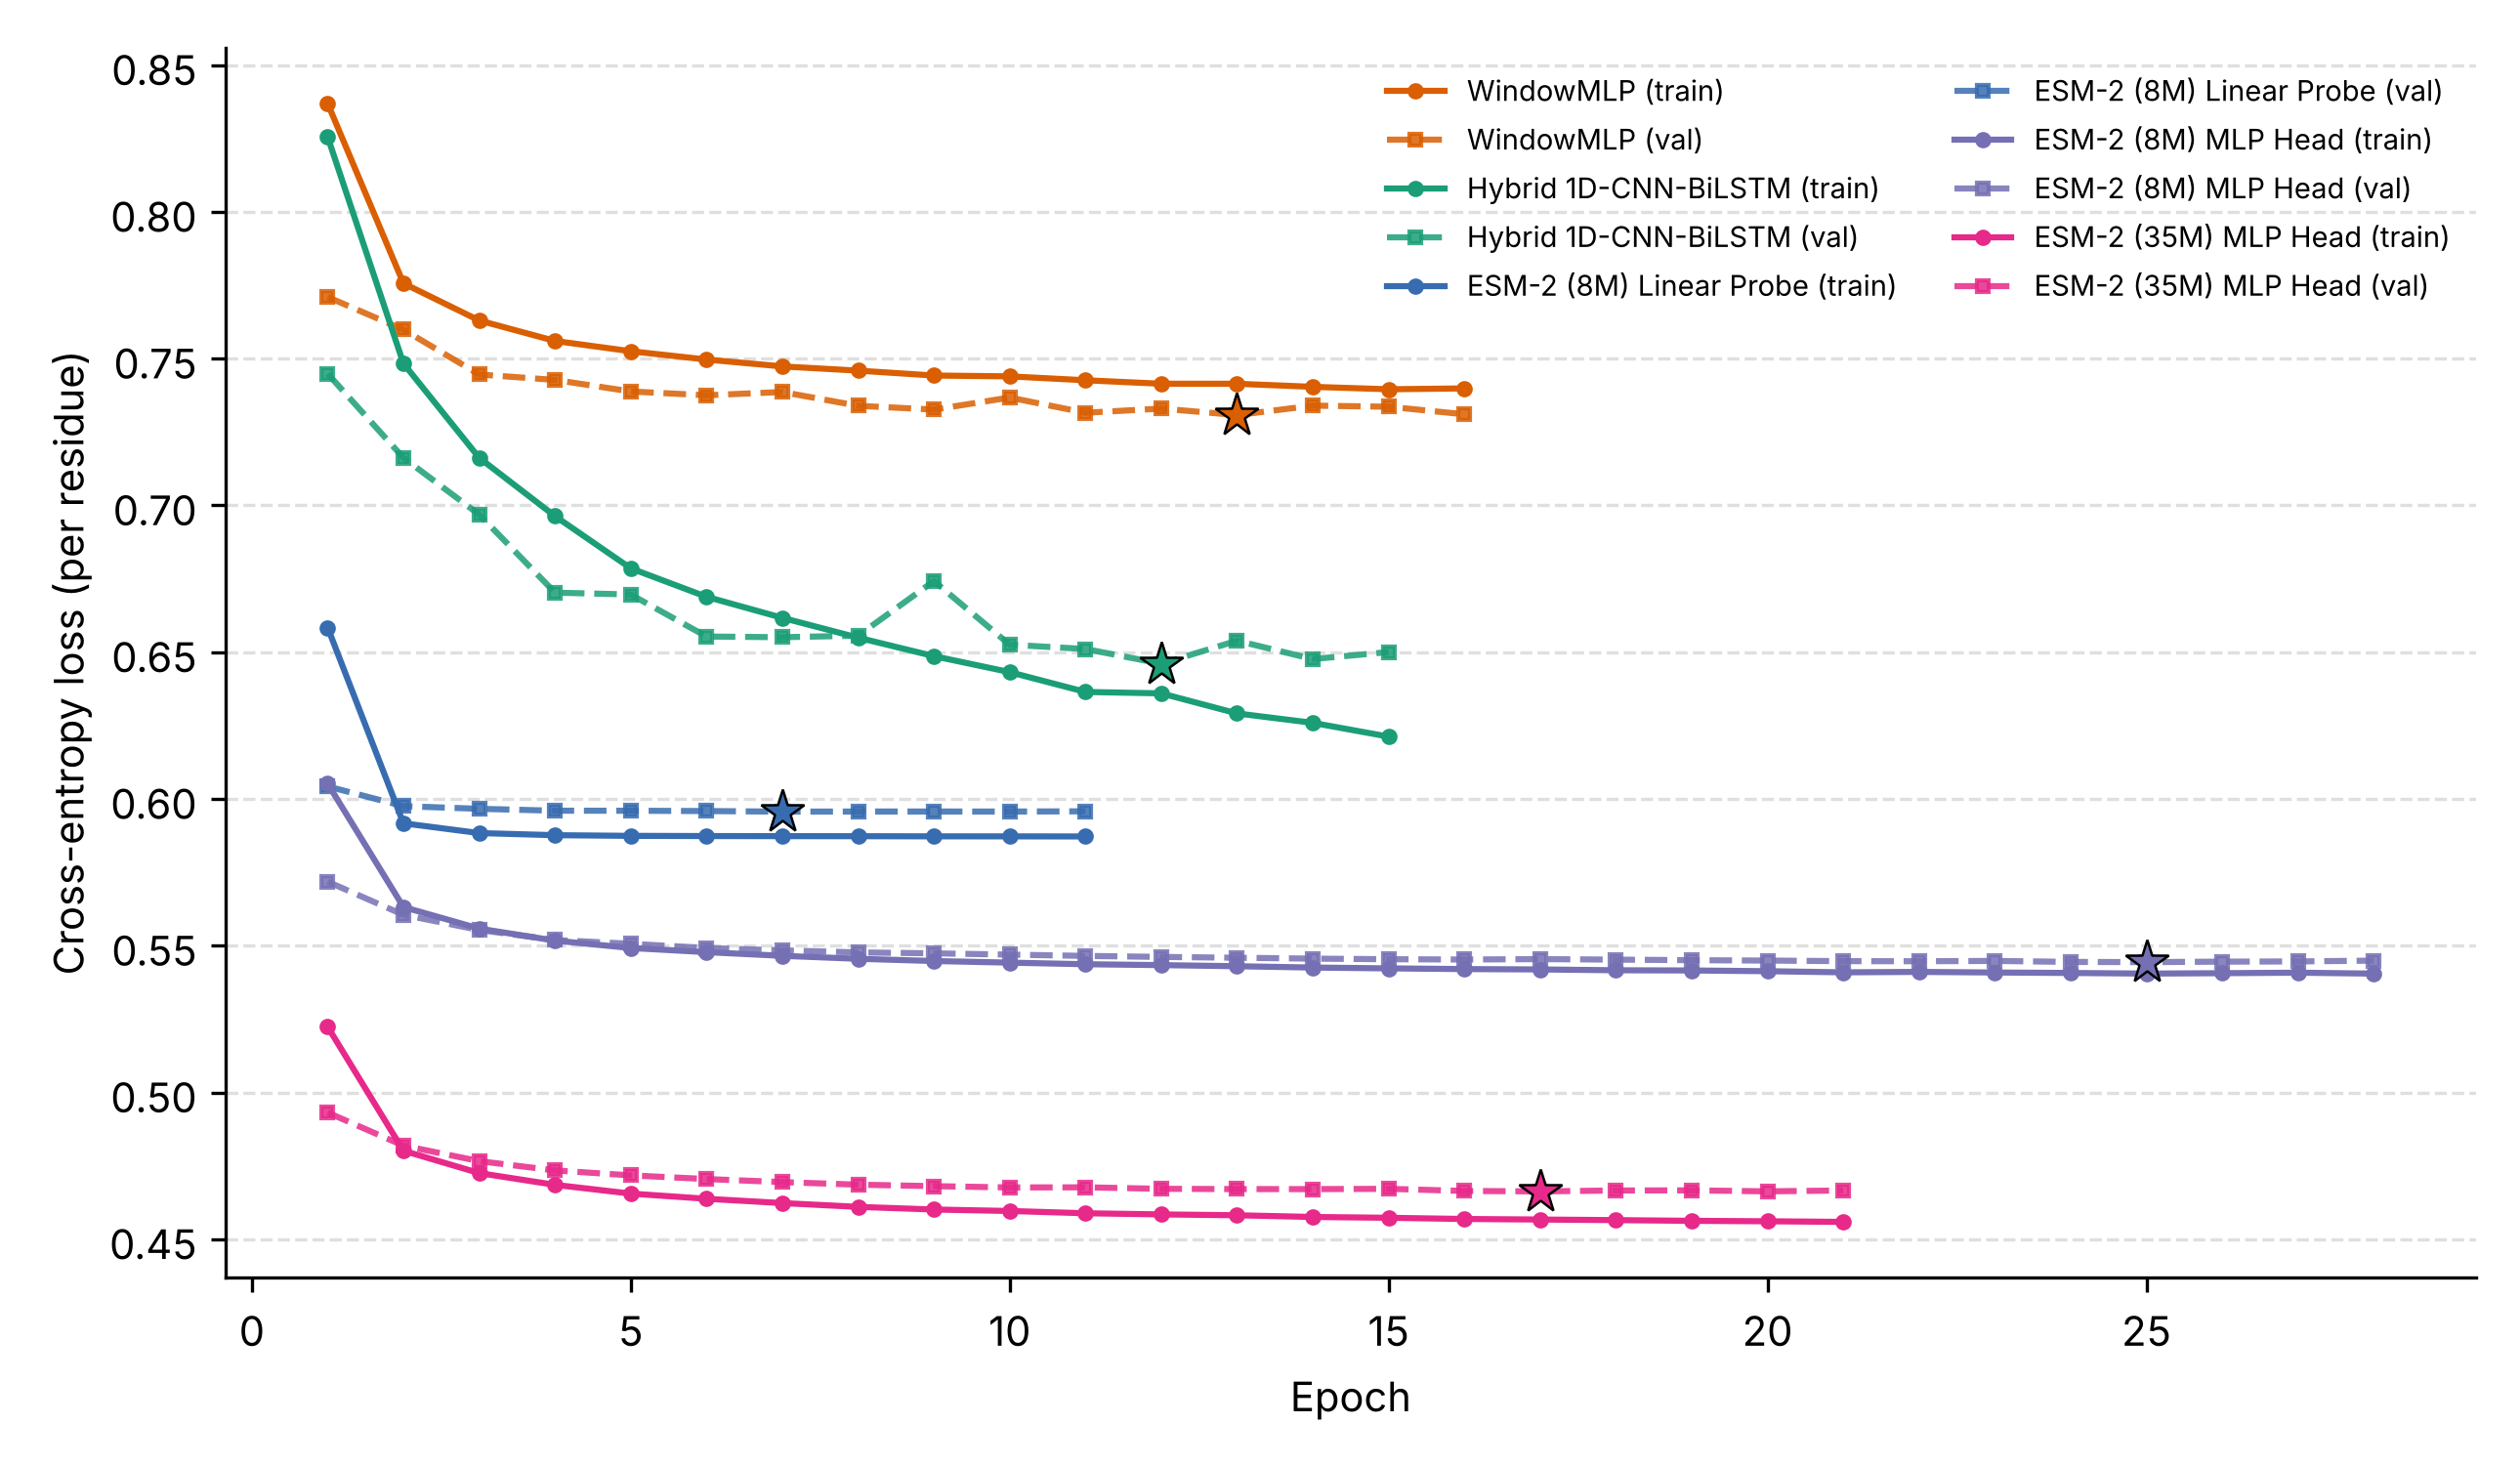
\includegraphics[width=0.98\linewidth]{results_real/fig_loss_curves.png}
\caption{Per-residue cross-entropy on the training (solid) and validation (dashed) sets for seed 42. Stars mark the selected (lowest validation loss) checkpoint.}
\label{fig:loss_curves}
\end{figure}

%======================================================================
\section{Discussion}
\label{sec:discussion}

\subsection{Context with published predictors}
Published results come from different training sets, evaluation masks and protocols, so they can only orient the reader. The closest reference point is the ProtTrans study~\citep{elnaggar2022prottrans}, which also trained on the NetSurfP-2.0 data and reported CASP12 $Q_3$ of 82.0\% for MSA-based NetSurfP-2.0, 81.4\% for ProtT5-XL-U50, 76.9\% for ESM-1b (650M parameters) and 75.8\% for ProtBert-BFD. On the same set, our frozen ESM-2 (35M) probe reached 74.84\% and ESM-2 (8M) 73.30\%. Small frozen ESM-2 models thus remain several points below large pLMs and MSA-based tools, and their appeal lies in cost rather than accuracy.

\subsection{Choosing a model under a CPU budget}
On a two-thread CPU, the frozen ESM-2 (8M) pipeline processed about 12 chains per second, the hybrid network about 70 and WindowMLP over 900. When language-model accuracy is needed and tens of milliseconds per chain are acceptable, ESM-2 (8M) with an MLP head is a reasonable default, and ESM-2 (35M) buys a further $\approx 4$ points for a fourfold increase in latency. When throughput matters most, the hybrid network is a compromise: it is $5.8\times$ faster than ESM-2 (8M) on CPU but recovers only $43.9\%$ of the gain of ESM-2 (8M) over WindowMLP, so the choice is a genuine trade-off rather than a free saving. Because the hybrid model was slower than ESM-2 (8M) on GPU, its advantage applies to CPU-only settings.

\subsection{Linear probe versus MLP head}
The MLP head added a consistent but modest $1.0$--$1.6$ points on four of five sets. This indicates that most of the three-state information in the last-layer ESM-2 (8M) embedding is linearly accessible, and that a small non-linear head mainly refines strand--coil and helix--coil boundaries (lower $\beta$--coil error). We did not test embeddings from intermediate layers, which are often more informative for structural probing, so these numbers are likely lower bounds for frozen ESM-2 features.

\subsection{Generalisation from CB513 to CASP targets}
Moving from CB513 to CASP14, $Q_3$ changed by $-1.41$ points for WindowMLP, $+0.11$ for the hybrid network, $-1.65$ for the ESM-2 (8M) linear probe, $-3.13$ for the ESM-2 (8M) MLP head and $-5.36$ for ESM-2 (35M); on CASP12 the corresponding changes were $-1.08$, $-1.62$, $-2.01$, $-2.62$ and $-5.28$. The pretrained models therefore lost more accuracy than the non-pretrained ones, and the loss grew with backbone size. One possible explanation is that CB513 chains, which are old and well represented in sequence databases, benefit from the pLM pretraining corpus (UniRef50), whereas newer CASP targets do not. Our data cannot establish this: CASP12 and CASP14 contain only 20 and 18 chains, the two benchmarks differ in composition, and TS115 and CASP13 did not show the same pattern as strongly. The observation nevertheless suggests that CB513 alone may overstate the advantage of pLM-based predictors, and that newer, larger temporally held-out benchmarks are needed.

\subsection{Limitations}
(i) A single train/validation split was used, and seeds varied only initialisation and data order. (ii) The CASP sets are small. (iii) Only last-layer embeddings and frozen backbones were studied; fine-tuning or layer selection would likely raise ESM-2 accuracy. (iv) The homology filter depends on MMseqs2 sensitivity, and filtering against the pLM pretraining corpus was not possible. (v) CPU timings were single runs on a shared cloud virtual machine, and peak inference memory was not measured; we report weight size instead.

%======================================================================
\section{Conclusion}
\label{sec:conclusion}
In a controlled benchmark with homology-filtered training data, frozen ESM-2 embeddings with small heads were the most accurate MSA-free predictors tested ($75.92\%$ and $80.12\%$ CB513 $Q_3$ for the 8M and 35M backbones), while a compact CNN--BiLSTM offered a $5.8\times$ CPU speed-up over ESM-2 (8M) at a cost of $4.47$ points. A non-linear head added a modest $1.6$ points over a linear probe. The larger drop of pretrained models from CB513 to recent CASP targets calls for caution when CB513 is the main benchmark for language-model-based predictors. All code, logs and per-residue predictions are released to allow the analysis to be reproduced and extended.

\section*{Declaration of Competing Interest}
The author declares no known competing financial interests or personal relationships that could have appeared to influence the work reported in this paper.

\section*{Declaration of Generative AI and AI-Assisted Technologies in the Writing Process}
During the preparation of this work, the author used large language model assistants for code drafting and review, text editing and formatting. After using these tools, the author reviewed and edited the content, ran all experiments, and takes full responsibility for the content of the publication.

\section*{Data and Code Availability}
The training and evaluation notebook, hyper-parameters, environment description, per-seed results, per-epoch losses, homology-filter hits and per-residue predictions are available at \url{https://github.com/ZAKI2828/pssp-efficiency-benchmark}. The datasets are publicly available from Hugging Face (\texttt{proteinea/secondary\_structure\_prediction}, DOI 10.57967/hf/1104).

\bibliographystyle{elsarticle-harv}
\begin{thebibliography}{17}

\bibitem[Buchan and Jones(2019)]{buchan2019psipred}
Buchan, D.W.A., Jones, D.T., 2019. The PSIPRED Protein Analysis Workbench: 20 years on. Nucleic Acids Res. 47 (W1), W402--W407.

\bibitem[Cuff and Barton(1999)]{cuff1999evaluation}
Cuff, J.A., Barton, G.J., 1999. Evaluation and improvement of multiple sequence methods for protein secondary structure prediction. Proteins 34 (4), 508--519.

\bibitem[Drozdetskiy et~al.(2015)]{drozdetskiy2015jpred4}
Drozdetskiy, A., Cole, C., Procter, J., Barton, G.J., 2015. JPred4: a protein secondary structure prediction server. Nucleic Acids Res. 43 (W1), W389--W394.

\bibitem[Elnaggar et~al.(2022)]{elnaggar2022prottrans}
Elnaggar, A., Heinzinger, M., Dallago, C., Rehawi, G., Wang, Y., Jones, L., Gibbs, T., Feher, T., Angerer, C., Steinegger, M., Bhowmik, D., Rost, B., 2022. ProtTrans: Toward understanding the language of life through self-supervised learning. IEEE Trans. Pattern Anal. Mach. Intell. 44 (10), 7112--7127. \url{https://doi.org/10.1109/TPAMI.2021.3095381}

\bibitem[H{\o}ie et~al.(2022)]{hoie2022netsurfp3}
H{\o}ie, M.H., Kiehl, E.N., Petersen, B., Nielsen, M., Winther, O., Nielsen, H., Hallgren, J., Marcatili, P., 2022. NetSurfP-3.0: accurate and fast prediction of protein structural features by protein language models and deep learning. Nucleic Acids Res. 50 (W1), W510--W515.

\bibitem[Jones(1999)]{jones1999protein}
Jones, D.T., 1999. Protein secondary structure prediction based on position-specific scoring matrices. J. Mol. Biol. 292 (2), 195--202.

\bibitem[Kabsch and Sander(1983)]{kabsch1983dictionary}
Kabsch, W., Sander, C., 1983. Dictionary of protein secondary structure: pattern recognition of hydrogen-bonded and geometrical features. Biopolymers 22 (12), 2577--2637.

\bibitem[Klausen et~al.(2019)]{klausen2019netsurfp}
Klausen, M.S., Jespersen, M.C., Nielsen, H., Jensen, K.K., Jurtz, V.I., S{\o}nderby, C.K., Sommer, M.O.A., Winther, O., Nielsen, M., Petersen, B., Marcatili, P., 2019. NetSurfP-2.0: Improved prediction of protein structural features by integrated deep learning. Proteins 87 (6), 520--527.

\bibitem[Lin et~al.(2023)]{lin2023evolutionary}
Lin, Z., Akin, H., Rao, R., Hie, B., et~al., 2023. Evolutionary-scale prediction of atomic-level protein structure with a language model. Science 379 (6637), 1123--1130.

\bibitem[Rives et~al.(2021)]{rives2021biological}
Rives, A., Meier, J., Sercu, T., Goyal, S., et~al., 2021. Biological structure and function emerge from scaling unsupervised learning to 250 million protein sequences. Proc. Natl. Acad. Sci. 118 (15), e2016239118.

\bibitem[Rost and Sander(1993)]{rost1993prediction}
Rost, B., Sander, C., 1993. Prediction of protein secondary structure at better than 70\% accuracy. J. Mol. Biol. 232 (2), 584--599.

\bibitem[Singh et~al.(2021)]{singh2021spot1d}
Singh, J., Litfin, T., Paliwal, K., Singh, J., Hanumanthappa, A.K., Zhou, Y., 2021. SPOT-1D-Single: improving the single-sequence-based prediction of protein secondary structure, backbone angles, solvent accessibility and half-sphere exposures using a large training set and ensembled deep learning. Bioinformatics 37 (20), 3464--3472.

\bibitem[Yang et~al.(2018)]{yang2018sixty}
Yang, Y., Gao, J., Wang, J., Heffernan, R., Hanson, J., Paliwal, K., Zhou, Y., 2018. Sixty-five years of the long march in protein secondary structure prediction: the final stretch? Brief. Bioinform. 19 (3), 482--494.

\bibitem[Zemla et~al.(1999)]{zemla1999modified}
Zemla, A., Venclovas, {\v{C}}., Fidelis, K., Rost, B., 1999. A modified definition of Sov, a segment-based measure for protein secondary structure prediction assessment. Proteins 34 (2), 220--223.

\end{thebibliography}

\end{document}
